\begin{figure}[t]
\centering
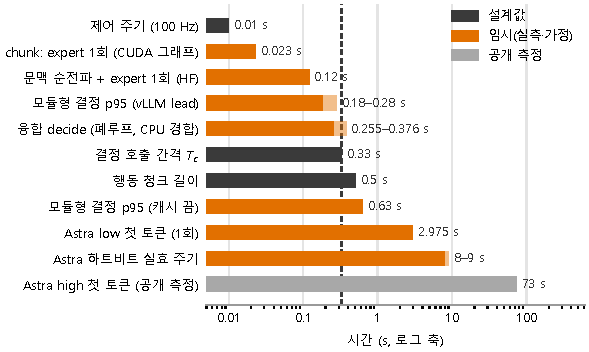
\includegraphics[width=\linewidth]{figures/latency_budget.pdf}
\caption{\textbf{층별 시간 예산(로그 축).} 검은 막대는 설계값, 주황 막대는 우리가 잰 임시 값 또는 가정값, 회색 막대는 공개 측정(Artificial Analysis, 2026-09-23, 우리가 잰 값 아님)이다. 모듈형 기준선의 vLLM 결정 호출(머리 + 손목, lead)은 호출 간격 $T_c=0.33$\,s 안에 들어온다. 융합 decide는 폐루프 파이프라인 시험에서 시뮬레이터와 CPU를 나눠 쓴 탓에 문턱을 넘기도 했고, chunk(expert, CUDA 그래프)는 수십 ms다. Astra는 그보다 한 자릿수 이상 느리므로 비동기로만 부른다. 주황 값은 모두 파이프라인 시험 값이다.}
\label{fig:latency}
\end{figure}
